\documentclass{article}
\usepackage[a4paper, total={6in, 8in}]{geometry}
\usepackage[utf8]{inputenc}
\usepackage{graphicx}
\usepackage{todonotes}

\usepackage[pdftex,
            pdfauthor={Pablo Botas},
            pdftitle={Developments}]{hyperref}

\title{Developments}
% \date{}
\author{Pablo Botas}

\begin{document}
\maketitle

\section{Algorithm}

This is the implemented algorithm:

\begin{enumerate}
    \item Read patient data
    \item Raytrace each spot in CT to get endpoint coordinates
    \begin{enumerate}
        \item Lose energy voxel-by-voxel
        \item Stop if outside of CT or no energy
    \end{enumerate}
    \item Probe vector field at the endpoint positions
    \item Apply VF at endpoints
    \item Apply VF at starting points keeping the same treatment plane
    \item Raytrace each spot in the CBCT to get endpoint coordinates
    \item Compare with warped endpoint calculated at step 5 (already along the same line, only depth difference)
    \item Assign 160MeV and move to the warped endpoint. Store the energy lost in it and its sign.
    \item Export tramp file for MC simulation
\end{enumerate}

The adaptation is then:
\begin{itemize}
    \item XY inside the treatment plane as given by the VF for each spot
    \item Energy as given by the range difference at last steps
\end{itemize}

Problems so far? Sure:
\newline

\todo[inline]{Is the VF probing done at the appropriate position?}
% \todo[inline]{How to fix the MHD/MHA output?}
\todo[inline]{Warping the endpoint and entrance point should not be done in parallel. When going further from the tramp center, a bigger angle should be applied!}
\todo[inline]{This effectively removes the layer organization in positions and energies.}

\begin{figure}[h]
    \centering
    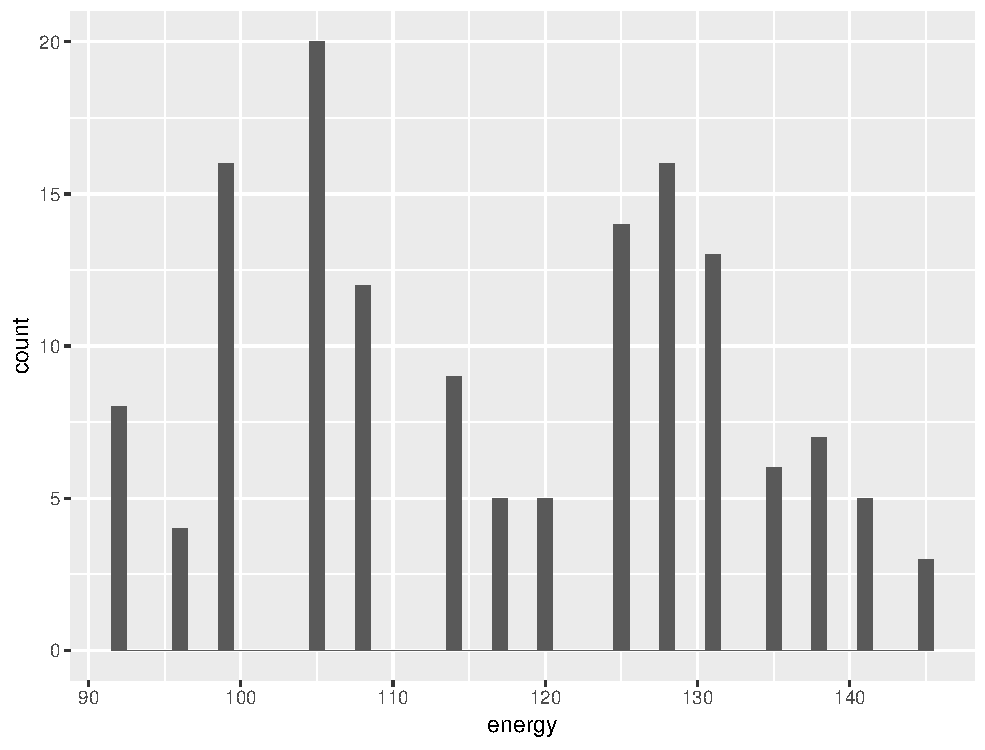
\includegraphics[width=0.49\textwidth]{energies_original.pdf}
    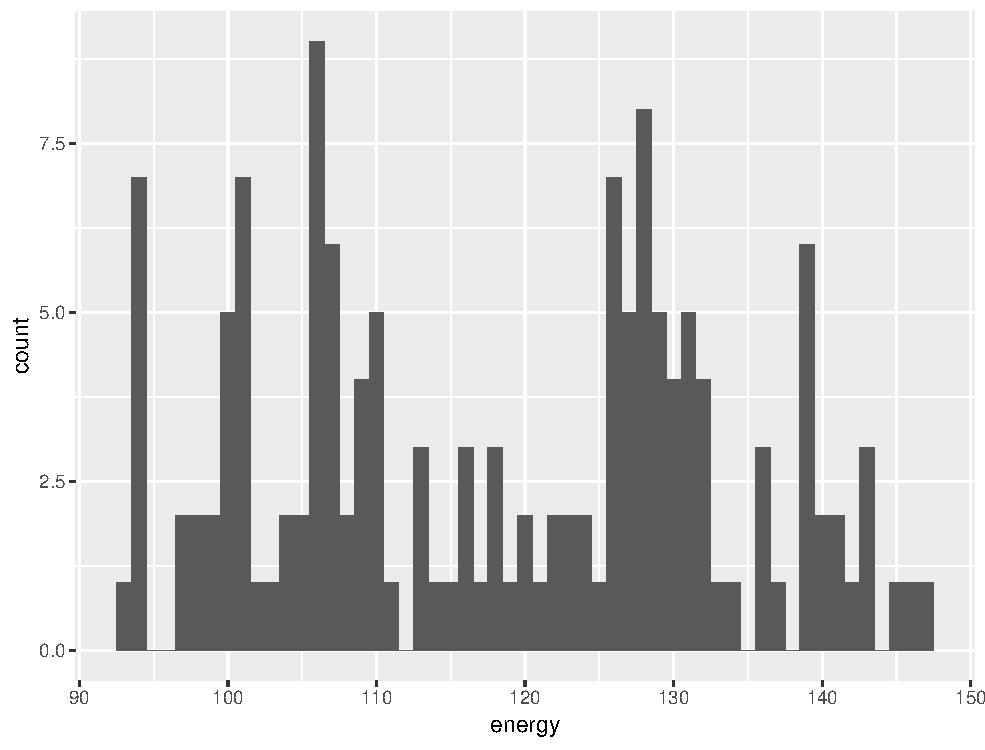
\includegraphics[width=0.49\textwidth]{energies_adapted.pdf}
    \caption{Histogram of the energy shifts.}
\end{figure}

\section{Ray Tracing validation}

The algorithm does a good job in predicting the range.

\begin{enumerate}
    \item A single ray is initialized per spot.
    \item The ray losses energy following the CSDA.
    \item When the ray has zero energy the endpoint is scored.
\end{enumerate}

\begin{figure}[h]
    \centering
    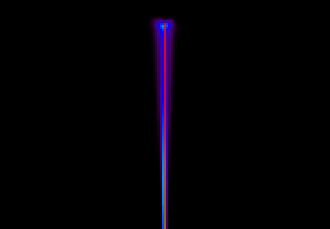
\includegraphics[width=0.49\textwidth]{beam.png}
    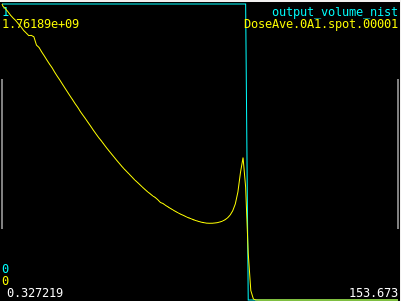
\includegraphics[width=0.49\textwidth]{profile.png}
    \caption{Beam with no $\sigma$ and $\epsilon$ in a patient (P15) and ray traced trajectory.}
\end{figure}

\section{Vector field probing}

It is done through Plastimatch, growing concerns here.

\section{Early results}

Applying the first version of the code to patient 1:

\begin{figure}[h]
    \centering
    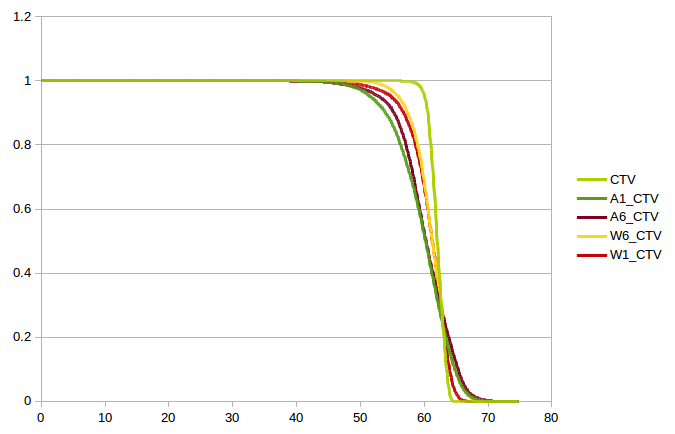
\includegraphics[width=0.6\textwidth]{pat1_init_dvh.png}
    \caption{DVH of different stages during treatment.}
\end{figure}

\end{document}